\documentclass{standalone}
\usepackage{circuitikz}
\usepackage{schemabloc}
\usetikzlibrary{positioning}

\begin{document}
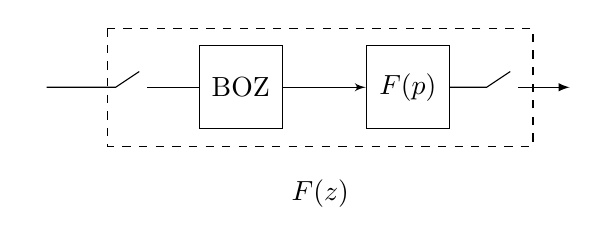
\begin{tikzpicture}
\sbEntree{E}
\draw[-] (E)--++(1,0) node (cnadroite) {} --++ (0.3,0.2) ; 
\sbBloc[3]{B1}{BOZ}{cna};
\draw[-,>=latex] (cnadroite)++(0.4,0) -- (B1);
\sbBloc[3]{B2}{$F(p)$}{B1};
\sbRelier[]{B1}{B2};
\draw[-] (B2)--++(1,0) node (candroite) {} --++ (0.3,0.2) ; 
\sbSortie[3]{S}{can};
\draw[->,>=latex] (candroite)++(0.4,0) -- (S);
\draw[dashed] (0.9,0.75) rectangle node[below,yshift=-3em] (){$F(z)$} (6.3,-0.75) ;
\end{tikzpicture}
\end{document}